\documentclass{beamer}
%pacchetti
\usepackage[T1]{fontenc}
\usepackage[utf8]{inputenc}
\usepackage{graphicx}
\usepackage[italian]{babel}
\usepackage{mathrsfs}
\usepackage{booktabs}
\usepackage{amsmath}
\usepackage{amsfonts}
\usepackage{amssymb}
\usepackage{amsbsy}
\usepackage{amsthm}
\usepackage{enumerate}
\usepackage{quoting}
\quotingsetup{font=small}
\usepackage{diagbox}
\usepackage{graphicx}
\usepackage{setspace}
\usepackage{float}
\usepackage{version}
\usepackage{multicol}
\usepackage{beamerfoils}

\usepackage[none]{hyphenat} %avoid hyphenation
\usepackage{xcolor} %to uset \textcolor
\usepackage{bbm} %funzione indicatrice
% end pacchetti

\usetheme[bgphoto]{polimi}

% Full instructions available at:
% https://github.com/elauksap/beamerthemepolimi

% Set custom font (requires to compile with XeLaTeX).
\usepackage{ifxetex}
\ifxetex
\usepackage{fontspec}
\setsansfont[Scale=0.9]{Arial}
\fi

\usepackage{lipsum}


\newcommand\mynum[1]{%
	\usebeamercolor{enumerate item}%
	\tikzset{beameritem/.style={circle,inner sep=0,minimum size=2ex,text=enumerate item.bg,fill=enumerate item.fg,font=\footnotesize}}%
	\tikz[baseline=(n.base)]\node(n)[beameritem]{#1};%
}


\title{Coupled Markov chains with applications to Approximate Bayesian Computation for model based clustering}
%\subtitle{Subtitle}
\author{E. Bertoni, M. Caldarini, F. Di Filippo, G. Gabrielli, E. Musiari}
\date{10 January 2022}


%Cose da fare

% Mettere biografia
% Mettere \pause e colori
% Sistemare il titolo e layout

\begin{document}

\begin{frame}
\maketitle
\end{frame}

	
\begin{section}{Introduction}

	\begin{frame}
		\frametitle{A complex problem}

 		\begin{minipage}{0.45\textwidth}
 			\begin{center}
 				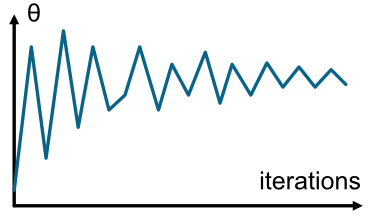
\includegraphics{img/markov_singola}
 			\end{center}
 		\end{minipage}
 		\hfill
 	 	\begin{minipage}{0.45\textwidth}
 	 		\begin{center}
 	 				
\includegraphics{img/likelihood_na}
 	 		\end{center}
 		\end{minipage}
 		
 		\vspace{0.5cm}

 		\begin{minipage}{0.45\textwidth}
 			\begin{center}
 				$\Downarrow$

 				\textbf{Unbiased Markov chain Monte Carlo methods with couplings}
 			\end{center}
 		\end{minipage} %}
 		\hfill
	 	\begin{minipage}{0.45\textwidth}
 			\begin{center}
 				$\Downarrow$
 				
 				 \textbf{Approximate Bayesian Computation}
 			\end{center}
 		\end{minipage} %}
 	 	
 	 	\vspace{0.2cm}
 	 	
 	 	\begin{minipage}{0.45\textwidth}
 	 		\begin{center}
 	 			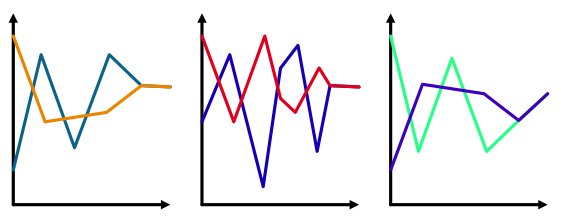
\includegraphics{img/markov_coupled_parallel}
 	 		\end{center}
 	 	\end{minipage}%}
 	 	\hfill
 	 	\begin{minipage}{0.45\textwidth}

 	 	\end{minipage}
 	 	
 	 	
 	 	
	\end{frame}

\end{section}
	
	
\begin{section}{Approximate Bayesian Computation}
	
	\begin{frame}[plain]{}
	\sectionpage
\end{frame}

%%%% (dire quale summary statistica usata, quale distanza usata, quale kernel)
\begin{frame}{ABC Metropolis Hastings}
\only<1,2,4,5,7> {
	\emph{Inputs:}
	\begin{itemize}
		\item a target posterior density $\pi(\theta | y_{obs}) \propto p(y_{obs}|\theta) \pi(\theta)$, consisting of a prior distribution $\pi(\theta)$ and a procedure of generating data under the model $p(y_{obs}|\theta)$;
		\item a Markov proposal density $g(\theta,\theta')$=$g(\theta' | \theta)$;
		\item an integer $N \textgreater0$;
		\only<1,4,5,7>{\item a kernel function $K_h(u)$ and a scale parameter $h > 0$;}
		\only<2>{\item  \textcolor{orange}{a kernel function $K_h(u)$ and a scale parameter $h > 0$};}
		\only<1,2,4,7>{\item a low dimensional vector of summary statistics $s=S(y)$.}
		\only<5>{\item \textcolor{orange}{a low dimensional vector of summary statistics $s=S(y)$}.}
	\end{itemize}
	
	\emph{Initialise:} \\
	repeat:
	\begin{enumerate}
		\item choose an initial parameter vector $\theta^{(0)}$ from the support of $\pi(\theta)$;
		\item generate $ y^{(0)} \sim p(y|\theta ^ {(0)})$ from the model and compute summary statistics $s^{(0)}=S(y^{(0)})$, until ${K_h(\parallel s^{(0)}-s_{obs}\parallel)} >0$.
	\end{enumerate}
}

\only<3> {

\begin{itemize}
	\item  a kernel function $K_h(u)$ and a scale parameter $h > 0$:
\end{itemize}

 
 $$\pi(\theta, y| y_{obs}) \propto \textcolor{orange}{\mathbbm{1}(\parallel y-y_{obs} \parallel \leq h)}p(y|\theta)\pi(\theta)$$
 \[ \Downarrow \]
 \[		\pi_{ABC}(\theta, y | y_{obs}) \propto \textcolor{orange}{K_h(u)}p(y|\theta)\pi(\theta)\]
 
 
 \vspace{0.7cm}
 Where $K$ is a standard smoothing kernel function and:
 \[ \textcolor{orange}{K_h(u)}  =  \frac{1}{h}  K \left( \frac{u}{h} \right), \quad \text{ with } \  u=\parallel y-y_{obs} \parallel \]
 
 

}

\only<6>{
	
	\begin{itemize}
		\item a low dimensional vector of summary statistics $s=S(y)$:
	\end{itemize}

\vspace{0.5cm}
	 $$ K_h(\parallel  y-y_{obs} \parallel ) $$
	\[ \Downarrow \]
	\[	K_h(\parallel S(y) - S(y_{obs}) \parallel )	\]
	

}

\only<8> {
	\emph{Sampling} for $i=1,...,N$:
	\begin{enumerate}
		\item generate candidate vector $\theta' \sim g(\theta^{(i-1)},\theta)$ from the proposal density $g$;
		\item generate $ y\,' \sim p(y|\theta')$ from the model and compute summary statistics  $s' = S(y\,')$;
		\item with probability $$\min \{ 1, \frac{K_h(\parallel s'-s_{obs}\parallel)   \pi(\theta')g(\theta',\theta^{(i-1)})}{K_h(\parallel s^{(i-1)}-s_{obs}\parallel)   \pi(\theta^{(i-1)})g(\theta^{(i-1)},\theta') } \}$$ 
		set $(\theta^{(i)},s^{(i)})=(	\theta',s')$. 
		Otherwise set  $(\theta^{(i)},s^{(i)})=(\theta^{(i-1)},s^{(i-1)})$.
	\end{enumerate}
	
	\emph{Output:}
	\begin{itemize}
		\item a set of correlated parameter vectors $\theta ^ {(1)},..., \theta ^ {(N)}$ from a Markov chain with stationary distribution $\pi_{ABC}(\theta |S_{obs})$.
	\end{itemize}
}
\end{frame}



\begin{frame}
\frametitle{Study case}
\only<1>{
\textbf{Summary statistic}: \\
\begin{center}
	Sample mean, vector of 9 quantiles
\end{center}

\textbf{Distance}: 
\begin{center}
	2-norm of the difference
\end{center}   %malanobis nel multivariato

\textbf{Kernel}: 
$$
K(u) = 
\frac{1}{\sqrt{2\pi}} e^{-\frac{1}{2}u^2}, 
\quad K_h(u) 
= \frac{K(\frac u h)}{h}
$$
%1/(np.sqrt(2*math.pi))np.exp(-1/2*u*2)
}
\only<2>{

\begin{block}{Model}
	\begin{center}
		$ Y_i | \mu \overset{iid}{\sim} \mathcal{N}(\mu, \sigma_{obs} ^2) $\\
		
		\vspace{0.3cm}
		
		$ \mu  \sim \mathcal{N}(\mu_0, \sigma_0^2)$
		
		$\mu_0 = 8, \quad \sigma^2_0 = 4$
	\end{center}
\end{block}

\begin{block}{Dataset}
	100 samples generated from a Gaussian distribution:
	\begin{center}
		$
		Y_{obs} \sim \mathcal{N}(\mu_{obs}, \sigma_{obs} ^2)
		$
		
		$
		\mu_{obs} = 10, \quad
		\sigma_{obs} ^2 = 3
		$
	\end{center}
\end{block}
}
\end{frame}


\begin{frame}{Results}

	{\small
		\textbf{Posterior distribution:}
		
		$$
		\mathcal{N}(\mu_n, \sigma^2_n), 
		\vspace{0.3cm}
		%\quad
		\mu_n 
		= \frac{1}{ \frac{1}{\sigma_0^2} + \frac{n}{\sigma_{obs}^2} } 
		\cdot \left(\frac{\mu_0}{\sigma_0^2} + \frac{\sum y_{obs}}{\sigma_{obs}^2}\right)
		\simeq 10.151,
		\vspace{0.3cm}
		%\quad
		\sigma^2_n
		= \frac{1}{ \frac{1}{\sigma_0^2} + \frac{n}{\sigma_{obs}^2} } 
		\simeq 0.0298
		$$
	}



\begin{minipage}{0.45\textwidth}
\begin{center}
	{\scriptsize \textbf{Sampling}}
	\includegraphics[width=\textwidth]{}
\end{center}
\end{minipage}
\hfill
\begin{minipage}{0.45\textwidth}
\begin{center}
	{\scriptsize \textbf{Sampling histogram with real distribution}}
	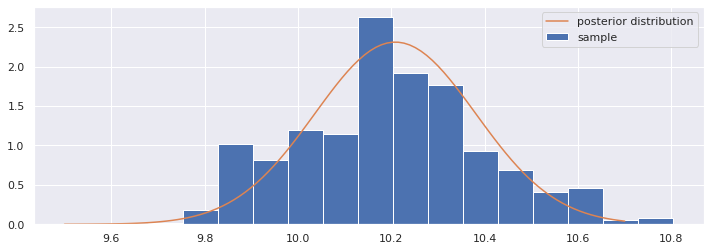
\includegraphics[width=\textwidth]{ABC_graphs/ABCunivgraphic}
\end{center}
\end{minipage}


\end{frame}


\begin{frame}{Results}
The same model using as summary statistic a vector of 9 quantiles:
\begin{center}
	\begin{minipage}{0.63\textwidth}
		\begin{center}
			{\scriptsize \textbf{Sampling}}
			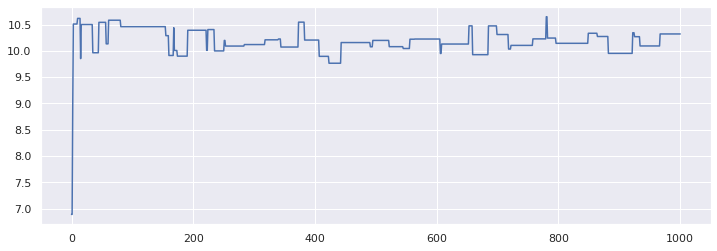
\includegraphics[width=\textwidth]{ABC_graphs/ABC_S1_1000iter}
		\end{center}
	\end{minipage}
	
	\vspace{0.2cm}
	
	\begin{minipage}{0.63\textwidth}
		\begin{center}
			{\scriptsize \textbf{Sampling histogram with real distribution}}
			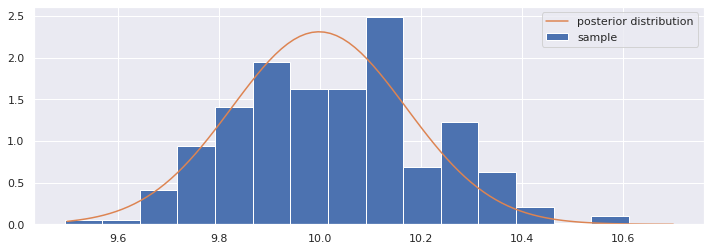
\includegraphics[width=\textwidth]{ABC_graphs/ABC_S1}
		\end{center}
	\end{minipage}
\end{center}
% grafici per un esempio univariato con summary mean -> e uno con quantili? (funzionava?)
\end{frame}


\end{section}
	
	\begin{section}{Conclusions}
	
    \begin{frame}[plain]{}
		\sectionpage
	\end{frame}

	\begin{frame}{Next steps}
	
		The next step will be the conclusion of the implementation of the MCMC with couplings and approximate bayesian computation on multivariate data.
		
		\vspace{0.5 cm}
		Further steps will be implementing the version with unknown variance and testing on more complex data.
		
		Finally, making comparisons with a standard MCMC algorithm.
	\end{frame}

	\begin{frame}{Bibliography}
		\nocite{*}
		\bibliographystyle{unsrt}
		\tiny{ \bibliography{refs_MCMC,refs_ABC} }

	
%				\begin{minipage}[t]{0.4\textwidth}
%			\footnotesize {Unbiased Markov chain Monte Carlo methods with couplings:}
%			\tiny { \bibliography{refs_MCMC} }
%		\end{minipage}
%		\hfill
%		\begin{minipage}[t]{0.4\textwidth}
%			\footnotesize {Approximate Bayesian computation:}
%			\tiny { \bibliography{refs_ABC} }
%		\end{minipage}

	\end{frame}
\end{section}


\end{document}
